%
%--- 
%-----------------------------------
\chapter{Magneto-Optical Trap}
\label{ch:MOT}
%-----------------------------------
%--- 
%

The magneto-optical trap (MOT) is a technique widely used in laser cooling experiments which allows both trapping and cooling of an atomic dilute gas. In this section, we shall approach the MOT theory \cite{krzysztof2010magneto, perrin2014doppler} considering the simplest transition $ J = 0 \rightarrow J = 1$, where $ J $ is the total angular momentum of the electronic state. To get an insight into the cooling and trapping mechanisms, we first discuss a simplified one-dimensional MOT (1D-MOT) assuming two counter-propagating laser beams and a linear magnetic field\footnote{A linear magnetic field is not a real magnetic field since it does not satisfy the Gauss's law for magnetism.}. Afterwards, we analyze the three-dimensional case assuming a standard arrangement with six counter-propagating laser beams. Finally, we introduce \textbf{narrow-line magneto-optical traps} (nMOTs) \cite{loftus2004narrow} by assuming an atomic transition with a natural linewidth (section \ref{sec:natural-broadening}) close to the photonic recoil.

% One-dimensinal case
%-----------------------------------
%
%-----------------------------------
\section{One-dimensional model}
\label{sec:one-dimensional-model}
%-----------------------------------
%

Let us consider a simplified one-dimensional model (1D-MOT) illustrated in figure \ref{fig:1D-MOT}. In this model, two counter-propagating laser beams of opposite circular polarization interact with an atom in the presence of a linear magnetic field $ \mathbf{B} = B_0 z \mathbf{e}_z $, where $ B_0 > 0 $ is the gradient magnitude. Both laser beams have the same angular frequency $ \omega $ and are tuned close to the transition $ J = 0 \rightarrow J = 1 $ whose angular frequency is $ \omega_0 $.

\begin{figure}[!ht]
	\centering
	\caption{1D-MOT}
	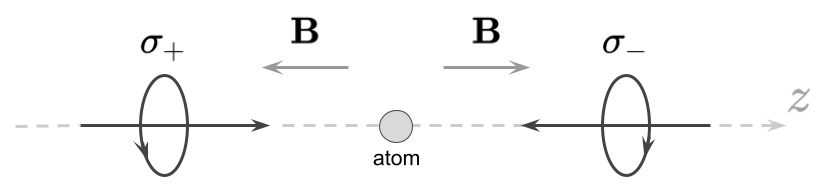
\includegraphics[width=0.7\textwidth]{USPSC-img/1D-MOT.png}
	\vspace{5pt}
	\legend{Simplified one-dimensional MOT composed of two counter-propagating laser beams and a linear magnetic field $ \mathbf{B} = B_0 z \mathbf{e}_z $, where $ B_0 > 0 $. We consider the $ \sigma_{+} $ and $ \sigma_{-} $ beams right-handed and left-handed polarized respectively. \\ Source: Author}
	\label{fig:1D-MOT}
	\vspace{-10pt}
\end{figure}

Disregarding the magnetic field, the transition is properly represented by a degenerate \textit{two-level system} whose energy difference is $ \hbar \omega_0 $. The presence of the magnetic field splits the energy level $ J = 1 $ into three different energy levels $ m_J = 0, \pm 1 $ such that the system turns into a \textit{four-level system} illustrated in figure \ref{fig:1D-MOT-Zeeman-splitting}. This effect is known as \textbf{Zeeman splitting} \cite[Section~7.4]{steck2007quantum}. Essentially, assuming a weak magnetic field\footnote{The quantity $ \mu_B B $, where $ B $ is the magnetic field magnitude, must be much lower than the spin-orbit coupling energy.}, there will be a effective detuning $ \delta_Z^{(m_J)} $ due to the \textbf{anomalous Zeeman effect} so that
\begin{equation}
	\delta_Z^{(m_J)} = - \beta g_{J} m_J z,\ \ \textrm{being}\ \ \beta \equiv \frac{\mu_B B_0}{\hbar},
	\label{eq:Zeeman-shift}
\end{equation}
where $ g_J $ is the \textit{Landé factor} and $ \mu_B $ is the Bohr magneton. The equation (\ref{eq:Zeeman-shift}) is also called \textbf{Zeeman shift}. It is relevant to notice that the detuning depends linearly on the position $ z $ so that $ \delta_Z^{(m_J)} \propto z $.

\begin{figure}[!ht]
	\centering
	\caption{Zeeman splitting in 1D-MOTs}
	\includegraphics[width=0.7\textwidth]{USPSC-img/1D-MOT-Zeeman-splitting.png}
	\vspace{5pt}
	\legend{Zeeman splitting of the transition $ J = 0 \rightarrow J = 1 $ in 1D-MOTs. When $ \mathbf{B} = 0 $ ($\mathbf{B}$ off), the atomic transition $ J = 0 \rightarrow J = 1 $ is described by a \textbf{degenerate two-level system}. However, when $ \mathbf{B} \neq 0 $ ($\mathbf{B}$ on), the same atomic transition is represented by a \textbf{four-level system} in which the excited states are energetically separeted by the Zeeman shift $ \delta_{Z}^{(\pm)} $. The energy scale was not plotted precisely to enhance the visibility.\\ Source: Author}
	\label{fig:1D-MOT-Zeeman-splitting}
\end{figure}

%-----------------------------------
\subsection{Cooling and trapping effect}
\label{sec:cooling-trapping-effect}
%-----------------------------------

Let us consider an arbitrary atom from an atomic cloud in a MOT neglecting interatomic interactions. Although the momentum exchange between atoms and light are quantized, we can evaluate the atom dynamics classically by assuming a mean force $ \mathbf{F}_{MOT} $, which is known as \textbf{semiclassical approach}. It is possible to obtain an analytical expression for $ \mathbf{F}_{MOT} $ under the \textbf{two-level system approximation}, which will be done in the next section \ref{sec:MOT-force}. Without this approximation, we must consider the interplay between optical pumping, photon scattering, Zeeman effect, and Doppler effect in multiple excited states. Therefore, the complexity of the problem will increase considerably. There are only a few articles \cite{prudnikov2015three, choi2008three, PhysRevA.49.4864} that approach this case.

We can be split $ \mathbf{F}_{MOT} $ into two components\footnote{In section \ref{sec:optical-forces}, we deduced both forces for the case of a two-level atom interacting with a single field.}: one exclusively associated with coherent transitions (absorption and \textit{stimulated} emission); and another associated with decoherence decays (absorption and \textit{spontaneous} emission). In weak atom-light coupling, stimulated emission is much less often than spontaneous emission. Therefore, $ \mathbf{F}_{MOT} $ is the \textbf{radiation pressure force}. Essentially, $ \mathbf{F}_{MOT} = (F_{+} - F_{-}) \mathbf{e}_z $, where $ F_{\pm} $ is related to the interaction between atom and the $ \sigma_{\pm} $-beam. Thus, $ F_{\pm} $ depends on the detuning $ \Delta_{\pm} $ so that the lower $ |\Delta_{\pm}| $, the greater $ F_{\pm} $. The detuning $ \Delta_{\pm} $ can be split into three detunings (figure \ref{fig:detuning-1D-MOT}) so that $ \Delta_{\pm} = \delta + \delta_Z^{\pm} + \delta_D^{\pm} $. These detunings are given by
\begin{itemize}
	\item \textit{Laser detuning} $ \delta = \omega - \omega_0 $: associated with the laser frequency $ \omega $ and the energy difference $ \omega_0 $ of the atomic transition. This detuning is the same for all transitions;

	\item \textit{Doppler shift} $ \delta_{D}^{(\pm)} = \mp k v $: associated with the atomic movement (see section \ref{sec:line-broadening-mechanisms});

	\item \textit{Zeeman shift} $ \delta_Z^{(\pm)} \propto \mp z $: associated with the Zeeman splitting. This detuning is given by the equation (\ref{eq:Zeeman-shift}).
\end{itemize}

\begin{figure}[!ht]
	\centering
	\caption{Detuning in 1D-MOT}
	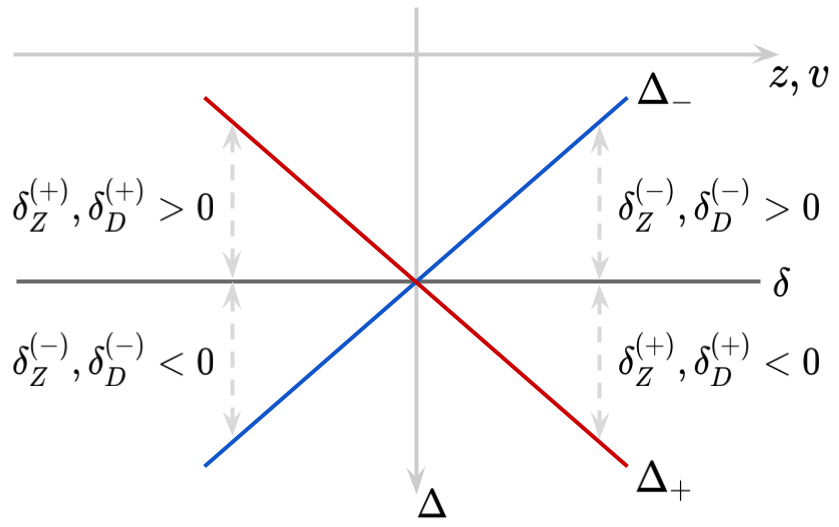
\includegraphics[width=0.55\textwidth]{USPSC-img/1D-MOT-detunings.png}
	\vspace{5pt}
	\legend{Laser detuning, Doppler shift, and Zeeman shift of a 1D-MOT in function of velocity $ v $ and position $ z $ assuming red-detuned laser beams ($ \delta < 0 $). \\ Source: Author}
	\label{fig:detuning-1D-MOT}
	\vspace{-20pt}
\end{figure}

Both Doppler shift and Zeeman shift increase linearly with the atom velocity and atom position respectively. Assuming red-detuned laser beams ($ \delta < 0 $) and $ v > 0 $, the probability of absorbing the $ \sigma_{\pm} $-beam decreases (increase) with $ v $ since $ |\Delta_{\pm}| $ increases (decreases). When $ v < 0 $, the opposite effect occurs. Therefore, the MOT force is opposite to the velocity $ v $ ($ \partial \mathbf{F}_{MOT} / \partial v < 0 $) such as a friction, which is is essentially a \textbf{cooling mechanism} also known as \textbf{Doppler cooling}. The Zeeman shift behaves the same in function of $ z $ such that the MOT force is also opposite to the position ($ \partial \mathbf{F}_{MOT} / \partial z < 0 $), which is essentially a \textbf{trapping mechanism}.

%-----------------------------------
\subsection{MOT Force}
\label{sec:MOT-force}
%-----------------------------------

We shall get deeper into the 1D-MOT analysis by quantifying the MOT force. As mentioned in section \ref{sec:cooling-trapping-effect}, obtain an analytical expression for the MOT forces in the general case is a complicated task. Although, we can obtain such analytical expression under two approximations:
\begin{itemize}
	\item By breaking the four-level system (figure \ref{fig:1D-MOT-Zeeman-splitting}) into three independent two-level systems illustrated in figure \ref{fig:independent-two-level-system}. That is a strong assumption in which the coherence effects between the Zeeman states, such as Raman-like transitions \cite[Section~9.8]{foot2005atomic}, are neglected;

	\item By assuming that the atom density operator $ \hat{\rho}(\mathbf{k}, -\mathbf{k}) $ related to the simultaneous interaction equals the sum of the density operators $ \hat{\rho}_{+}(\mathbf{k}) $ and $ \hat{\rho}_{-}(-\mathbf{k}) $ associated with the individual interactions, which is essentially a superposition ($ \hat{\rho} = \hat{\rho}_{+} + \hat{\rho}_{-} $). This approximation relies on the perturbation theory in first and second-order \cite[Chapter~7]{berman2011principles}. 
\end{itemize}

Both approximations are valid in the regime of weak atom-light coupling so that the total detuning is higher than the power-broadened linewidth.

\begin{figure}[!ht]
	\centering
	\caption{Assumption of independent two-level systems}
	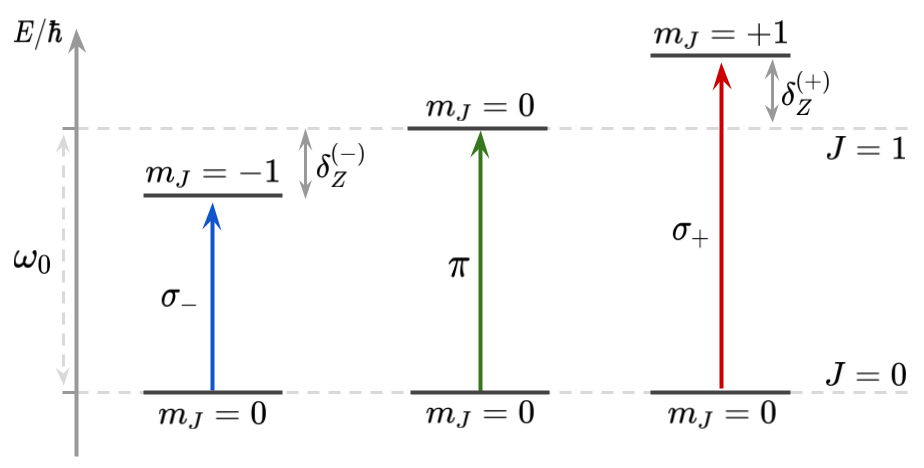
\includegraphics[width=0.6\textwidth]{USPSC-img/Independent-two-level-system.png}
	\legend{Breaking of the four-level system into three independent two-level systems.\\ Source: Author}
	\label{fig:independent-two-level-system}
\end{figure}

Since there are only right-handed and left-handed polarized beams, there will only $ \sigma_{\pm} $-transitions. Therefore, the components $ F_{+} $ and $ F_{-} $ associated with the $ \sigma_{+} $ and $ \sigma_{-} $ transitions respectively are independent radiation pressure forces given by (see section \ref{sec:optical-forces})
\begin{equation}
	F_{\pm}(z, v) = \pm \hbar k \frac{\Gamma}{2} \frac{s_0}{1 + s_0 + 4(\Delta_{\pm} / \Gamma)^2},
	\label{eq:1D-MOT-force-components}
\end{equation}
where $ \Delta_{\pm} = \delta + \delta_{Z}^{(\pm)} + \delta_{D}^{(\pm)} $, $ s_0 $ is the saturation parameter, and $ \Gamma $ is the natural linewidth\footnote{The natural linewidth depends on the energy difference between the states, which is slightly different in each transition. However, this energy difference is much lower than $ \hbar \omega_0 $ such that the natural linewidth is approximately $ \Gamma $.} of the transition $ J = 0 \rightarrow J = 1 $. Assuming low velocities ($ |kv| \ll |\delta| $) and positions close to the magnetic field centre ($ |z| \ll |\delta| $), the MOT force is essentially linear with $ z $ and $ v $ as illustrated in figure \ref{fig:MOT-force}. Hence, we can expand $ F_{MOT} $ about $ z = 0 $ and $ v = 0 $ so that
\begin{equation}
	F_{MOT}(z, v) \simeq F_{MOT}(0, 0) + z \frac{\partial F_{MOT}}{\partial z}(0, 0) + v \frac{\partial F_{MOT}}{\partial v}(0, 0),
	\label{eq:MOT-force-Taylor-expansion}
\end{equation}

\begin{figure}[!ht]
	\centering
	\caption{MOT force}
	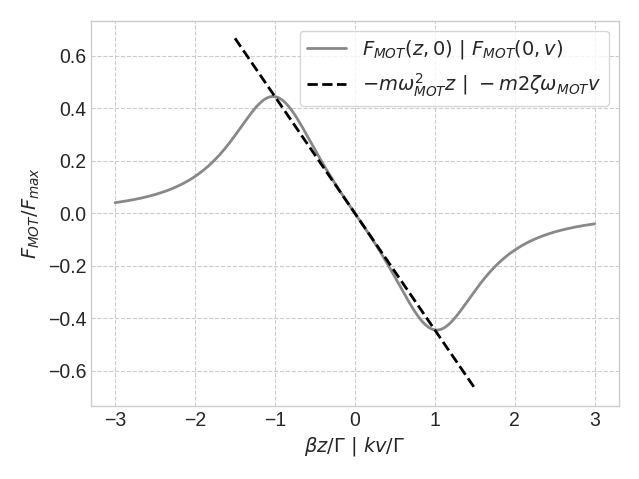
\includegraphics[width=0.5\textwidth]{USPSC-img/MOT_force.png}
	\legend{Plotting of the MOT force $ F_{MOT} $ for $ v = 0 $ ($ z = 0 $) in function of $ \beta z / \Gamma $ ($ k v / \Gamma $) considering the transition $ {}^{1}S_0 \rightarrow {}^{1}P_1 $ of the $ {}^{88}Sr $ for $ \delta = - \Gamma $ and $ s_0 = 1 $. The dashed line in the graph is the MOT force assuming $ |\beta z| \ll |\delta| $ ($ |kv| \ll |\delta| $).\\ Source: Author}
	\label{fig:MOT-force}
\end{figure}

Rearranging the terms of equation (\ref{eq:MOT-force-Taylor-expansion}), we obtain
\begin{gather}
	\frac{d^2 z}{dt^2} + 2\zeta \omega_{MOT} \frac{d z}{d t} + \omega_{MOT}^2 z = 0,
	\label{eq:damped-harmonic-oscillation-1D-MOT}
	\\
	\omega_{MOT}^2 \equiv - \frac{1}{m} \frac{8 \hbar k \beta g_J s_0 (\delta / \Gamma)}{[1 + s_0 + 4(\delta / \Gamma)^2]^2},\ \ \textrm{and}\ \ \zeta \equiv \frac{k}{2\beta g_J} \omega_{MOT},
	\label{eq:constants-equation-of-motion-1D-MOT}
\end{gather}
where $ m $ is the atomic mass. The quantity $ \omega_{MOT} $ has unit of frequency and $ \zeta $ is a dimensionless quantity. Also, $ \omega_{MOT}^2 $ is a positive real value since we are assuming red-detuned lasers, which means $ \delta < 0 $ in equation \ref{eq:constants-equation-of-motion-1D-MOT}. The equation of motion (\ref{eq:damped-harmonic-oscillation-1D-MOT}) describes a \textit{damped harmonic oscillation} of which $ \omega_{MOT} $ is the \textit{undamped frequency} and $ \zeta $ is the \textit{damping ratio}. Therefore, the atom is trapped by the restoring force $ - m \omega_{MOT}^2 z $, being limited to move in a restricted region (\textbf{trapping mechanism}). Furthermore, the atom loses energy due to the damping $ 2 \zeta \omega_{MOT} v $ can be understood as a \textbf{cooling mechanism}.

%-----------------------------------
%

% Three-dimensional case
%-----------------------------------
%
%-----------------------------------
\section{Three-dimensional case}
\label{eq:three-dimensional-case}
%-----------------------------------
%
\begin{wrapfigure}{l}{0.5\textwidth}
	\centering
	\caption{Standard 3D-MOT arrangement}
	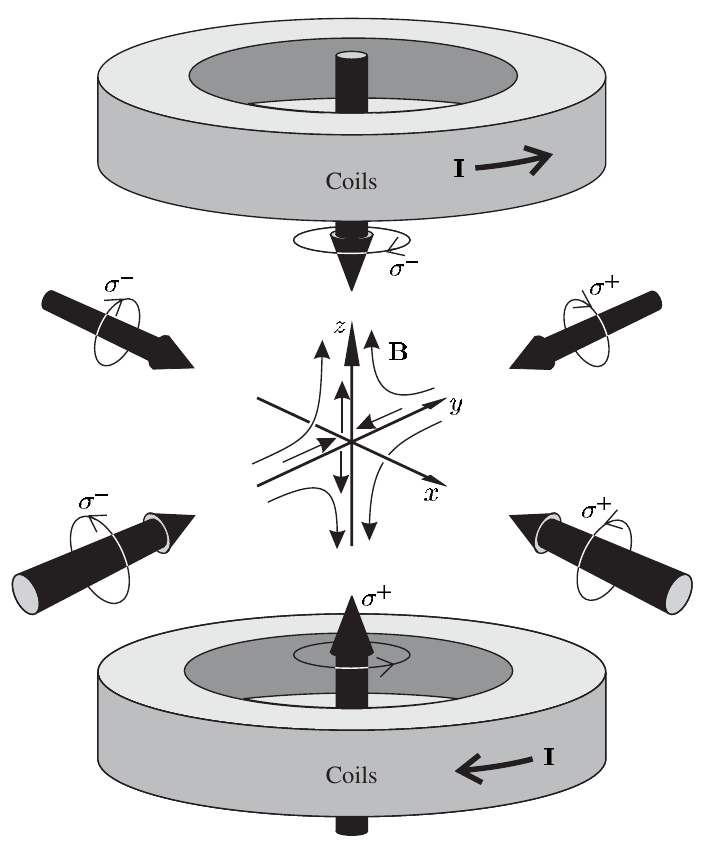
\includegraphics[width=0.45\textwidth]{USPSC-img/standard-3D-MOT-arrangement.png}
	\legend{Standard arrangement of MOT composed of three orthogonal pairs of counter propagating laser beams with opposite circular polarization and coils in anti-Helmholtz configuration, which produces a magnetic quadrupole field. \\ Source: \cite[Figure~9.9]{foot2005atomic}}
	\label{fig:standard-3D-MOT-arrangement}
	\vspace{-20pt}
\end{wrapfigure}
Let us assume the standard 3D-MOT arrangement illustrated in figure \ref{fig:standard-3D-MOT-arrangement}. An atom, free to move along all Cartesian axes, interacts with \textit{three pairs} of counter-propagating laser beams with opposite circular polarization and a magnetic quadrupole field $ \mathbf{B} $. In a first attempt, we can naturally extend the 1D-MOT theory into a 3D theory considering that each laser beam yields a radiation pressure force given by equation (\ref{eq:1D-MOT-force-components}). Nevertheless, the quantization axis ($z$-axis) must match the direction of the field $ \mathbf{B} $ to proper evaluate the Zeeman shift, which implies that each laser beam polarization depends on the atomic position. This is not a concern in the 1D-MOT since the magnetic field has a fixed direction. Therefore, a theoretical description of the 3D-MOT \cite{prudnikov2015three} encounters considerable difficult due to the spatial-dependence of the quantization axis. Regardless the theoretical complications, the cooling and trapping effects of MOTs are widely confirmed for many alkali \cite{raab1987trapping, katori1999magneto, zachorowski1998magneto} and lanthanide \cite{maier2014narrow, miyazawa2021narrow, frisch2012narrow}. Also, in this thesis, we could demonstrate both effects for dysprosium and strontium atoms through a stochastic simulation. Moreover, it is possible to estimate temperature and also atomic cloud size.

%-----------------------------------
\subsection{Limit temperature in Doppler cooling}
\label{sec:Doppler-temperature-limit}
%-----------------------------------

Let us consider a equilibrium atomic position close to the magnetic field centre. In this case, the Zeeman shift becomes negligible compared to the Doppler shift ($ \delta_{Z} \ll \delta_{D} $) such that a defined quantization axis is no longer required. \footnote{Essentially, we are proposing the treatment of a MOT as an \textbf{optical molasses}, which is a similar technique to only cool an atomic dilute gas based upon \textit{Doppler cooling}.} Also, we suppose weak atom-light couplings in which the laser detuning are grater than the power-broadened linewidth. Thus, the interaction between each laser beam and the atom is independent and it is described by two-level dynamics. In this situation, the MOT force is given by
\begin{equation}
	\mathbf{F}_{MOT}(\mathbf{v}) = \frac{\hbar k \Gamma s_0}{2} \sum_{n = 1}^{3} \left( \frac{1}{1 + s_0 + 4[\delta - k (\mathbf{v} \cdot \mathbf{e}_n)]^2 / \Gamma^2} - \frac{1}{1 + s_0 + 4[\delta + k (\mathbf{v} \cdot \mathbf{e}_n)]^2 / \Gamma^2} \right)\mathbf{e}_{n},
\end{equation}
where $ \{ \mathbf{e}_1, \mathbf{e}_2, \mathbf{e}_3 \}$ is the Cartesian basis. We are assuming all laser beams with the same saturation parameter $ s_0 $, wavevector magnitude $ k $, and detuning $ \delta $. For low velocities $ v $ such that $ kv \ll \delta $, we can expand the MOT force around $ \mathbf{v} = 0 $ so that $ \mathbf{F}_{MOT} \simeq - \gamma \mathbf{v} $,
\begin{equation}
	\gamma = - \frac{8 \hbar k^2 s_0 (\delta / \Gamma)}{[1 + s_0 + 4(\delta / \Gamma)^2]^2}.
\end{equation}
Assuming red-detuned laser beams ($ \delta < 0 $), we have $ \gamma > 0 $ and then $ \mathbf{F}_{MOT} $ describes a friction force. Hence, the velocity vanishes after a time as long as $ 1 / \gamma $ and then the final temperature should be zero. However, the $ \mathbf{F}_{MOT} $ is an average and therefore we must take its fluctuations into account. These fluctuations are associate with the Brownian atomic motion due to spontaneous emission, which yields a \textit{heating process}. Therefore, a finite temperature is set by the balance between cooling and heating mechanisms. 

Let us considering a cycle of $ N $ 

%-----------------------------------
\subsection{Atomic cloud size}
\label{sec:MOT-cloud-size}
%-----------------------------------
%-----------------------------------
%

% Narrow Line Magneto-Optical Trap
%-----------------------------------
%
%-----------------------------------
\newpage
\section{Narrow-line magneto-optical trap}
%-----------------------------------
%

\begin{wrapfigure}{l}{0.4\textwidth}
    \centering
    \vspace{-10px}
    \caption{Atomic cloud shape in nMOTs for small laser intensities.}
    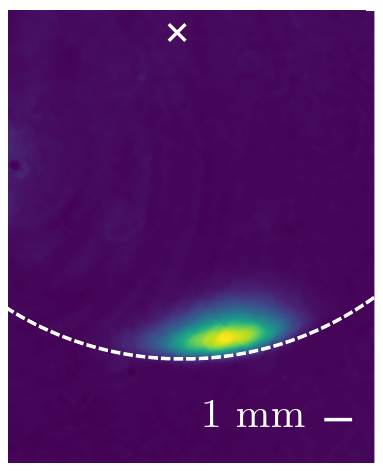
\includegraphics[width=0.3\textwidth]{USPSC-img/atomic_cloud_shape_in_nMOTs.png}
    \legend{Typical \textit{in situ} absorption image of an atomic sample in a nMOT. \\ Source: \cite{dreon2017optical}}
    \label{fig:atomic-cloud-shape-nMOTs}
    \vspace{-10px}
\end{wrapfigure}

In previous sections, we have been neglecting the gravity effect on the MOT parameters. This assumption is valid when the MOT force is much higher than gravity. The maximum radiation pressure force on an atom is $ \hbar k \Gamma / 2 $ from equation (\ref{eq:1D-MOT-force-components}). Therefore, the ratio between the maximum radiation pressure force and gravity is
\begin{equation}
    R \equiv \frac{\hbar k \Gamma}{2 m g},
    \label{eq:gravity-radiation-force-ratio}
\end{equation}
where $ m $ is the atomic mass and $ g $ is the gravitation acceleration. Usually, $ R $ is on the order of $ 10^5 $. Hence, the gravity force is negligible since the radiation pressure force is much higher. However, the lower $ \Gamma $, the higher the gravity effect so that for $ \Gamma \sim\ \textrm{kHz} $, the ratio (\ref{eq:gravity-radiation-force-ratio}) approaches values on the order of $ 10 $. In this case, the centre of mass moves towards the gravity direction such that, for small laser intensities, the atoms gather on the bottom of the surface of an ellipsoid as illustrated in figure \ref{fig:atomic-cloud-shape-nMOTs}.

Furthermore, $ \Gamma $ also defines the average number of scattering events per time (\textbf{scattering rate}) so that the lower $ \Gamma $, the fewer the number of events in a determined time interval. We have been analysing the atoms dynamics classically through the optical forces, which assumes that there are a large number of momentum exchange in a small period of time. In this condition, we can average out a force. That is not satisfied when $ \Gamma $ is sufficient smaller. In this case, we must include the discrete momentum exchange in the analysis and then treat the dynamics quantum mechanically. To quantify the range of $ \Gamma $ in which this happens, let us define the ratio given by
\begin{equation}
    \eta = \frac{\Gamma}{\omega_R} = \frac{m \lambda^2 \Gamma}{2\pi^2 \hbar} =
    \label{eq:narrowness}
\end{equation}
where $ \hbar \omega_R $ is the kinetic energy $ (\hbar k)^2 / (2 m) $ gain by the atom when it absorbs an photon with the momentum $ \hbar k $, $ h $ is the Planck constant, and $ \lambda = 2\pi/k $ is the wavelength. This energy is known as \textbf{photonic recoil}. When $ \eta \leq 1 $, one scattering event is able to detune the atom-light interaction. A MOT whose $ \eta \sim 1 $ or less is known as \textbf{narrow-line magneto-optical trap} (nMOT), whereas a MOT whose $ \eta \gg 1 $ is known as \textbf{broad-line magneto-optical trap}. We shall call the ratio (\ref{eq:narrowness}) as \textbf{narrowness}.


%-----------------------------------
\subsection{Operating regimes}
\label{sec:nMOT-operating-regimes}
%-----------------------------------

Four quantities play a crucial role in nMOTs operating: the saturation parameter $ s_0 $, the laser detuning $ \delta $, the natural linewidth $ \Gamma $, and the photonic recoil $ \omega_R $. We can combined $ s_0 $ and $ \Gamma $ in a single quantity known as \textbf{power-broadened linewidth} $ \Gamma' \equiv \Gamma \sqrt{1 + s_0} $, which is the natural energy scale of the atom-light interaction due to the power-broadening mechanism (section \ref{sec:line-broadening-mechanisms}). Furthermore, we can summarize those quantities in two essential quantities that characterized nMOTs:
\begin{itemize}
    \item ($ \eta' \equiv \Gamma' / \omega_R $): it defines the relevance of single scattering events to the the atom-light interaction taking the natural energy scale into account. Hence, $ \eta' $ is more accurate than $ \eta $;
    \item ($ \delta' \equiv \delta / \Gamma' $): it defines the coupling strength between atom and light normalized by the natural energy scale of the interaction.
\end{itemize}
When $ \eta' \gg 1 $, the semiclassical approach is suitable since the photonic recoil is much lower than the natural energy scale and, therefore, the scattering events can be averaged out. There are three nMOTs regimes:
\begin{enumerate}
    \item[I] \textbf{Doppler regime} ($ \eta' \gg 1 $ and $ |\delta'| < 1 $): in this regime, gravity is negligible so that the atomic cloud is ellipsoidal;
    \item[II] \textbf{Power-broadened regime} ($ \eta' \gg 1 $ and $ |\delta'| > 1 $): In this regime, gravity is comparable to the radiation pressure forces such that the atomic cloud centre of mass sags to vertical positions.
    \item[III] \textbf{Quantum regime} ($ \eta' \sim 1 $): in this regime, the photonic recoil is the natural energy scale and, therefore, the quantum physics governs the nMOT dynamics.
\end{enumerate}

%-----------------------------------
\subsection{Centre of mass of the atomic cloud}
\label{sec:nMOT-centre-of-mass}
%-----------------------------------

We can estimate the centre of mass of the atomic cloud in the power-broadened regime by assuming that all radiation pressure forces on an atom balance each other in all directions except in the gravity direction $ \hat{z} $. In this direction, the radiation pressure forces $ F_{\pm} $ balance with the gravity force as illustrated in figure \ref{fig:forces-diagram-trapped-atom-nMOT-power-broadened-regime}.
\begin{figure}[!ht]
    \centering
    \caption{Forces diagram of a trapped atom}
    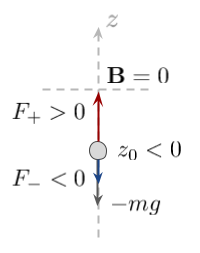
\includegraphics[width=0.17\textwidth]{USPSC-img/centre_of_mass_power_broadened_regime.png}
    \legend{Forces diagram of a trapped atom in a power-broadened nMOT. \\ Source: author}
    \label{fig:forces-diagram-trapped-atom-nMOT-power-broadened-regime}
    \vspace{-10px}
\end{figure}
Thus, a trapped atom is restricted to be in a region where the magnetic field components perpendicular to $ z $ is zero, otherwise there will be unbalance between forces in those direction due to the Zeeman shift (see section \ref{sec:cooling-trapping-effect}). The average position of a trapped atom must be $ \vec{r} = z_0 \hat{z} $ so that its dynamics is well described by the one-dimensional model presented in section \ref{sec:one-dimensional-model}. From equations (\ref{eq:1D-MOT-force-components}), we obtain the following equation of motion
\begin{equation}
    \hbar k \frac{\Gamma}{2} s_0 \left( \frac{1}{1 + s_0 + 4(\Delta_{+} / \Gamma)^2} - \frac{1}{1 + s_0 + 4(\Delta_{-} / \Gamma)^2}  \right) - mg = 0.
    \label{eq:equation-motion-1D-model-under-gravity}
\end{equation}
We must impose $ |\Delta_{+}| < |\Delta_{-}| $ to ensure a solution to the equation (\ref{eq:equation-motion-1D-model-under-gravity}). Neglecting the Doppler shift ($ \delta_{D}^{(\pm)} = 0 $), and assuming red-detuned lasers\footnote{This assumption is necessary to create a trapping environment as discussed in \ref{sec:cooling-trapping-effect}.} ($ \delta < 0 $), we obtain $ z_0 < 0 $, which means the centre of mass will be located below the magnetic field origin. Let us consider $ |\delta| \gg 1 $ so that $ |\Delta_{+}| \gg |\Delta_{-}| $. In this condition, $ F_{-} $ is negligible. Hence, we can approximate the equation (\ref{eq:equation-motion-1D-model-under-gravity}) to
\begin{equation}
    \hbar k \frac{\Gamma}{2} s_0 \left( \frac{1}{1 + s_0 + 4[(\delta + \delta_{Z}^{(+)}) / \Gamma]^2}\right) - mg = 0.
\end{equation}
We have been assuming the transition $ J = 0 \longrightarrow J = 1 $ such that $ \delta_Z^{(+)} = - \beta g_J m_J z $. However, the transition can happen between any transition $ J = j \longrightarrow J = j + 1$, where $ j \geq 0 $. To take it into account, we must consider
\begin{equation}
     \delta_Z^{(+)} = - \beta \chi z_0,\ \textrm{being}\ \chi \equiv (g_J - g_J') j > 0,
     \label{eq:zeeman-shift-generic-transition}
\end{equation}
where $ g_J' $ and $ g_J $ are the \textit{Landé factors} of the excited and ground states respectively. The equation (\ref{eq:zeeman-shift-generic-transition}) is valid when the transitions only happens between the states $ m_J = -j $ and $ m_J = -j + 1 $. Isolating $ z_0 $, we obtain
\begin{equation}
    z_0 = - \frac{1}{\beta \chi} \left(\delta + \frac{\Gamma}{2} \sqrt{\frac{h \Gamma s_0}{2 \lambda m g} - 1 - s_0} \right)
    \label{eq:centre-of-mass-power-broadened-regime}
\end{equation}
The equation (\ref{eq:centre-of-mass-power-broadened-regime}) is only valid when the centre of mass is sufficient below the magnetic field origin to match all the assumptions described above and in section \ref{sec:MOT-force}.

%-----------------------------------
%